\documentclass[crop,tikz,12pt]{standalone}

\usepackage{tikz}
\usetikzlibrary{matrix}
\usetikzlibrary{arrows.meta}
\usetikzlibrary{calc}
\usetikzlibrary{fit}

\def\term{\sffamily}

\definecolor{bg1}{RGB}{244,231,195}
\definecolor{bg2}{RGB}{234,204,161}
\definecolor{l1}{RGB}{209,148,106}


\begin{document}

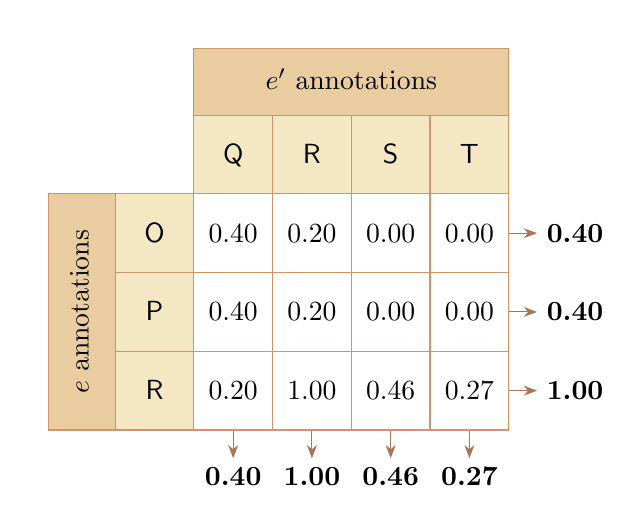
\begin{tikzpicture} [
    f/.style={draw=l1!80!black,-{Stealth}},
    headerb/.style={
        fill=bg2,
        inner sep=-0.5\pgflinewidth,
        outer sep=0pt,
        draw=l1
    }
]

\matrix (table) [
    matrix of nodes,
    row sep=-\pgflinewidth,
    column sep=-\pgflinewidth,
    row 2/.style={font=\sffamily,nodes={fill=bg1}},
    column 2/.style={font=\sffamily,nodes={fill=bg1}},
    nodes={
        align=center, minimum size=1cm,
        text depth=0.5ex,text height=2ex,
        text width=2em,
        draw=l1
    },
    ndf/.style={draw=none, fill=none}
]{
    \node [ndf] (t11) {}; &
    \node [ndf] (t12) {}; &
    \node [ndf] (t13) {}; &
    \node [ndf] (t14) {}; &
    \node [ndf] (t15) {}; &
    \node [ndf] (t16) {}; \\
    %
    \node [ndf] (t21) {}; &
    \node [ndf] (t22) {}; &
    \node       (t23) {Q}; &
    \node       (t24) {R}; &
    \node       (t25) {S}; &
    \node       (t26) {T}; \\
    %
    \node [ndf] (t31) {}; &
    \node       (t32) {O}; &
    \node       (t33) {0.40}; &
    \node       (t34) {0.20}; &
    \node       (t35) {0.00}; &
    \node       (t36) {0.00}; \\
    %
    \node [ndf] (t41) {}; &
    \node       (t42) {P}; &
    \node       (t43) {0.40}; &
    \node       (t44) {0.20}; &
    \node       (t45) {0.00}; &
    \node       (t46) {0.00}; \\
    %
    \node [ndf] (t51) {}; &
    \node       (t52) {R}; &
    \node       (t53) {0.20}; &
    \node       (t54) {1.00}; &
    \node       (t55) {0.46}; &
    \node       (t56) {0.27}; \\
};

\node [fit={($(t31.north west)+(1ex,0)$)(t51.south east)},headerb](e1header){};
\node [xshift=-1pt,anchor=center,rotate=90] at (e1header.center)
    {$e$ annotations};

\node [fit={($(t13.north west)-(0,1ex)$)(t16.south east)},headerb](e2header){};
\node [yshift=1pt,anchor=center] at (e2header.center) {$e'$ annotations};

\draw [f] (t53.south) -- ++(0,-10pt) node [font=\bfseries,anchor=north] {0.40};
\draw [f] (t54.south) -- ++(0,-10pt) node [font=\bfseries,anchor=north] {1.00};
\draw [f] (t55.south) -- ++(0,-10pt) node [font=\bfseries,anchor=north] {0.46};
\draw [f] (t56.south) -- ++(0,-10pt) node [font=\bfseries,anchor=north] {0.27};

\draw [f] (t36.east) -- ++(10pt,0) node [font=\bfseries,anchor=west] {0.40};
\draw [f] (t46.east) -- ++(10pt,0) node [font=\bfseries,anchor=west] {0.40};
\draw [f] (t56.east) -- ++(10pt,0) node [font=\bfseries,anchor=west] {1.00};

%\draw [f] ()

\end{tikzpicture}

\end{document}
